\section{The Two-Body Problem}
This investigation treats the motion of spacecraft in heliocentric space, specifically when they
are far from planets and moons, as a 2-body Problem, governed by a single gravitational force. This
section provides a brief overview of key aspects of 2BP dynamics, Keplerian orbital elements, and
Kepler's Equation. For a more comprehensive derivation of the 2BP, refer to Chapters 1 and 2 of
Vallado's \emph{Fundamentals of Astrodynamics and Applications}\cite{Vallado:2013}. Additionally,
Canales highlights the background information relevant to understanding the transfer methodologies
presented in this analysis\cite{Canales:2021b}.

\subsection{Equations of Motion}
The 2BP involves two point masses\textemdash a primary body and a spacecraft\textemdash that exert
gravitational forces on each other. Since no external forces act on this system, the center of mass
of the bodies moves at a constant velocity and serves as the origin for an inertial coordinate
frame. In this inertial frame, the gravitational force that the primary body exerts on the
spacecraft, denoted as $\Fbar_{g_{P\rightarrow s/c}}$, is expressed as:
\begin{equation}
    \Fbar_{g_{P\rightarrow s/c}}=-\frac{Gm_{P}m_{s/c}}{r_{P\rightarrow s/c}^{3}}\rbar_{P\rightarrow s/c},
    \label{eq:gravity}
\end{equation}
where $G$ is the universal gravitational constant (6.67384x10$^{-20}$ kN*km$^{2}$/kg$^{2}$),
$m_{P}$ and $m_{S}$ are the masses of the primary body and spacecraft, respectively,
$r_{P\rightarrow s/c}$ is the distance from the primary body to the spacecraft, and
$\rbar_{P\rightarrow s/c}=\rbar_{s/c}-\rbar_{P}$ is the position vector from the primary body to
the spacecraft in the inertial frame, as illustrated in \cref{fig:2BP}.

\begin{figure}[ht]
    \centering
    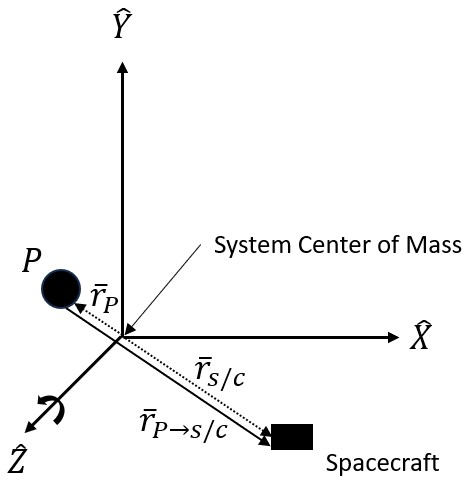
\includegraphics[width=0.5\textwidth]{figures/TBP.jpg}
    \caption{Two-body problem in a barycentric inertial frame.}
    \label{fig:2BP}
\end{figure}

Assuming that the mass of the spacecraft is negligible compared to the mass of the primary body,
the nonlinear relative equation of motion for the 2BP is derived\cite{Vallado:2013,Canales:2021b}:
\begin{equation}
    \rbarddot_{P\rightarrow s/c}=-\frac{\mu_{2BP}}{r_{P\rightarrow s/c}^{3}}\rbar_{P\rightarrow s/c},
    \label{eq:TBPEoM}
\end{equation}
where $\rbarddot_{P\rightarrow s/c}$ is the inertial acceleration of the spacecraft relative to the
primary body and $\mu_{2BP}=Gm_{P}$. This vector equation can also be expressed as $\Xhat$,
$\Yhat$, and $\Zhat$ scalar equations in the inertial frame:
\begin{equation}
    \Xddot=-\frac{\mu_{2BP}}{r_{P\rightarrow s/c}^{3}}(X_{s/c}-X_{P}),
    \label{eq:TBPEoMX}
\end{equation}
\begin{equation}
    \Yddot=-\frac{\mu_{2BP}}{r_{P\rightarrow s/c}^{3}}(Y_{s/c}-Y_{P}),
    \label{eq:TBPEoMY}
\end{equation}
\begin{equation}
    \Zddot=-\frac{\mu_{2BP}}{r_{P\rightarrow s/c}^{3}}(Z_{s/c}-Z_{P}).
    \label{eq:TBPEoMZ}
\end{equation}

\subsection{Conic Sections}
Instead of relying on numerical propagation of the nonlinear equations of motion, spacecraft motion
in the 2BP can be effectively represented analytically using conic sections. This section provides
a concise overview of conic motion in the 2BP.

Two essential constants characterize conic orbits: specific angular momentum $\ambar$ and specific
mechanical energy $\mathcal{E}$:
\begin{equation}
    \ambar=\rbar_{P\rightarrow s/c}\times\rbardot_{P\rightarrow s/c},
    \label{eq:angularmomentum}
\end{equation}
\begin{equation}
    \mathcal{E}=\frac{v_{P\rightarrow s/c}^{2}}{2}-\frac{\mu_{2BP}}{r_{P\rightarrow s/c}},
    \label{eq:energy}
\end{equation}
where $v_{P\rightarrow s/c}=||\rbardot_{P\rightarrow s/c}||_{2}$ is the spacecraft velocity in the
inertial frame relative to the primary body.

Kepler's first law, asserting that orbital motion is conic, provides the trajectory equation for
the 2BP:
\begin{equation}
    r_{P\rightarrow s/c}=\frac{a(1-e^{2})}{1+e\cos(\theta)},
    \label{eq:trajectory}
\end{equation}
where $a$ represents the orbit semimajor axis, $e$ is the orbit eccentricity, and $\theta$ denotes
the orbit true anomaly. These three elements will be elaborated upon in a later subsection.
\cref{eq:trajectory} can also be employed to compute the periapsis and apoapsis distances, $r_{p}$
and $r_{a}$ respectively:
\begin{equation}
    r_{p}=a(1-e),
    \label{eq:periapsis}
\end{equation}
\begin{equation}
    r_{a}=a(1+e).
    \label{eq:apoapsis}
\end{equation}

The eccentricity can also be used to determine the type of conic section:
\begin{itemize}
    \item   $e=0$: Circular orbit (a special case of an ellipse).
    \item   $0<e<1$: Elliptical orbit.
    \item   $e=1$: Parabola.
    \item   $e>1$: Hyperbola.
\end{itemize}
This investigation focuses on circles and ellipses with $0\leq e<1$.

Similarly, Kepler's third law provides the orbit period $\mathbb{P}$ and, consequently, the mean
motion $n$:
\begin{equation}
    \mathbb{P}=2\pi\sqrt{\frac{a^{3}}{\mu_{2BP}}},
    \label{eq:period}
\end{equation}
\begin{equation}
    n=\frac{2\pi}{\mathbb{P}}=\sqrt{\frac{\mu_{2BP}}{a^{3}}}.
    \label{eq:meanmotion}
\end{equation}

\subsection{Keplerian Orbital Elements}
Instead of specifying the six-dimensional state of a spacecraft in a 2BP elliptical orbit using
Cartesian coordinates, six orbital elements can be employed to articulate the size, shape,
orientation, and current location along the orbit. In addition to the semimajor axis $a$ and
eccentricity $e$, which were introduced earlier and describe the size and shape of the ellipse,
three angles characterize the orientation of the orbit with respect to an inertial frame, as
depicted in \cref{fig:orbitalElements}:
\begin{itemize}
    \item \textbf{Inclination} $i$ signifies the tilt of the orbital plane relative to the inertial
    $\Xhat_{Ec}\Yhat_{Ec}$-plane.
    \item \textbf{Right ascension of the ascending node} (RAAN) $\Omega$ denotes the angle between
    the $\Xhat_{Ec}$-axis and the ascending node, where the orbit crosses the
    $\Xhat_{Ec}\Yhat_{Ec}$-plane in the positive $\Zhat_{Ec}$ direction.
    \item \textbf{Argument of periapsis} $\omega$ is the angle between the ascending node and the
    periapsis.
\end{itemize}
Finally, the true anomaly $\theta$ defines the spacecraft's position relative to the orbit's
periapsis.

\begin{figure}[ht]
    \centering
    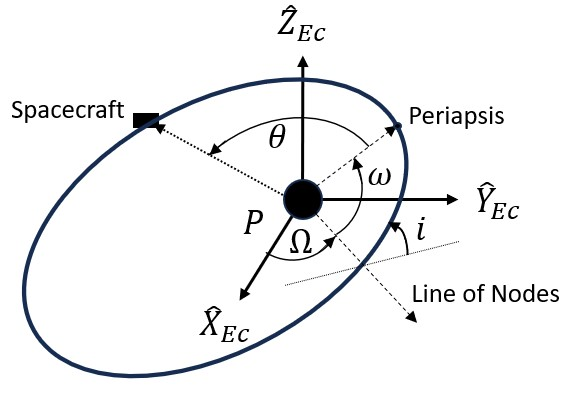
\includegraphics[width=0.5\textwidth]{figures/OrbitalElements.jpg}
    \caption{Orientation and location along an orbit in an inertial frame using Keplerian orbital elements.}
    \label{fig:orbitalElements}
\end{figure}

\subsubsection{Cartesian state to Keplerian orbital elements}
To convert from a Cartesian state vector to Keplerian orbital elements, start by calculating the
inclination from angular momentum:
\begin{equation}
    i=\arccos(\frac{h_{Z}}{||\ambar||})
    \label{eq:inclination}
\end{equation}
Using the node vector $\nbar$:
\begin{equation}
    \nbar=\Zhat_{Ec}\times\ambar,
    \label{eq:nodes}
\end{equation}
the RAAN becomes:
\begin{equation}
    \Omega=\begin{cases}\arccos(\frac{n_{X}}{||\nbar||})&n_{Y}\geq0\cr2\pi-\arccos(\frac{n_{X}}{||\nbar||})&n_{Y}<0\end{cases}.
    \label{RAAN}
\end{equation}
The eccentricity vector $\ebar$ is also calculated from the angular momentum:
\begin{equation}
    \ebar=\frac{\rbardot_{P\rightarrow s/c}\times\ambar}{\mu_{2BP}}-\frac{\rbar_{P\rightarrow s/c}}{r_{P\rightarrow s/c}},
    \label{eq:eccentricityvector}
\end{equation}
and
\begin{equation}
    e=||\ebar||.
    \label{eq:eccentricity}
\end{equation}
The remaining three orbital elements are calculated as follows:
\begin{equation}
    a=\frac{||\ambar||}{\mu_{2BP}(1-e^{2})},
    \label{eq:semimajoraxis}
\end{equation}
\begin{equation}
    \omega=\begin{cases}\arccos(\frac{\nbar\cdot\ebar}{||\nbar||e})&e_{Z}\geq0\cr2\pi-\arccos(\frac{\nbar\cdot\ebar}{||\nbar||e})&e_{Z}<0\end{cases},
    \label{eq:argumentofperiapsis}
\end{equation}
\begin{equation}
    \theta=\begin{cases}\arccos(\frac{\ebar\cdot\rbar_{P\rightarrow s/c}}{er_{P\rightarrow s/c}})&v_{r}\geq0\cr2\pi-\arccos(\frac{\ebar\cdot\rbar_{P\rightarrow s/c}}{er_{P\rightarrow s/c}})&v_{r}<0\end{cases},
    \label{eq:trueanomaly}
\end{equation}
where
\begin{equation}
    v_{r}=\frac{\rbardot_{P\rightarrow s/c}\cdot\rbar_{P\rightarrow s/c}}{r_{P\rightarrow s/c}}.
    \label{eq:radialvelocity}
\end{equation}

\subsubsection{Keplerian orbital elements to Cartesian state}
Similarly, the Cartesian state vector can be obtained from the Keplerian orbital elements. First,
the eccentric anomaly $E$ is needed, which is the angle made by the eccentricity vector pointing to
periapsis and the vector from the center of the ellipse to the point directly above the spacecraft
location (perpendicular to the eccentricity vector) on an auxiliary circle drawn tangent to the
ellipse. The eccentric anomaly and the auxiliary circle are illustrated in \cref{fig:auxCircle}, along
with the eccentricity vector and semimajor axis.

\begin{figure}[ht]
    \centering
    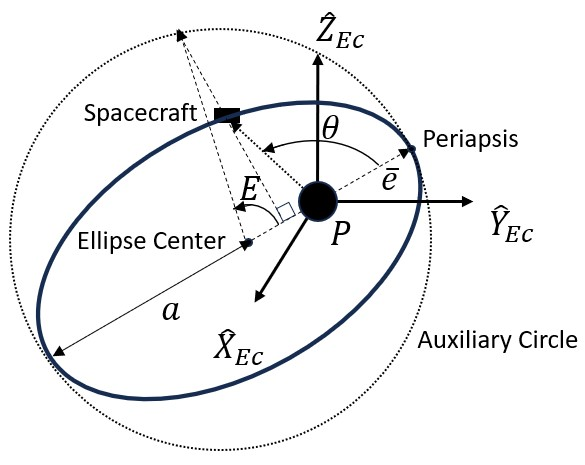
\includegraphics[width=0.5\textwidth]{figures/AuxCircle.jpg}
    \caption{Definition of eccentric anomaly and the auxiliary circle.}
    \label{fig:auxCircle}
\end{figure}

The eccentric anomaly can be related to the true anomaly,
\begin{equation}
    E=\arctan(\frac{\sqrt{1-e^{2}}\sin(\theta)}{e+\cos(\theta)}),
    \label{eq:eccentricanomaly}
\end{equation}
which can then be used to calculate the distance from the primary:
\begin{equation}
    r_{P\rightarrow s/c}=a(1-e\cos(E)).
    \label{eq:circularradius}
\end{equation}
This can be used to generate position and velocity magnitude vectors:
\begin{equation}
    \rbar_{0}=\begin{bmatrix}r_{P\rightarrow s/c}\cos(\theta)\cr r_{P\rightarrow s/c}\sin(\theta)\cr0\end{bmatrix},
    \label{eq:circularpositionvector}
\end{equation}
\begin{equation}
    \rbardot_{0}=\sqrt{\frac{\mu_{2BP}a}{r_{P\rightarrow s/c}}}\begin{bmatrix}-\sin(E)\cr\sqrt{1-e^{2}}\cos(E)\cr0\end{bmatrix}.
    \label{eq:circularvelocityvector}
\end{equation}
These vectors will need to be rotated relative to the inertial frame axes according to the
inclination, RAAN, and argument of periapsis:
\begin{equation}
    C=\begin{bmatrix}\cos(\Omega)\cos(\omega)-\cos(i)\sin(\Omega)\sin(\omega)&-\cos(\Omega)\sin(\omega)-\cos(i)\sin(\Omega)\cos(\omega)&0\cr\sin(\Omega)\cos(\omega)+\cos(i)\cos(\Omega)\sin(\omega)&-\sin(\Omega)\sin(omega)+\cos(i)\cos(\Omega)\cos(\omega)&0\cr\sin(i)\sin(\omega)&\sin(i)\cos(\omega)&0\end{bmatrix},
    \label{eq:elementrotation}
\end{equation}
\begin{equation}
    \rbar_{P\rightarrow s/c}=C\rbar_{0},
    \label{eq:positionvector}
\end{equation}
\begin{equation}
    \rbardot_{P\rightarrow s/c}=C\rbardot_{0}.
    \label{eq:velocityvector}
\end{equation}

\subsection{Kepler's Equation}
If the difference in true anomaly between two points on an orbit is known, Kepler's equation
becomes a valuable tool for calculating the time-of-flight between these points. The mean anomaly
$M$ serves as a measure of how much of the orbit has been traversed past periapsis with respect to
time:
\begin{equation}
    M=\frac{2\pi(t-t_{p})}{\mathbb{P}},
    \label{eq:meananomaly}
\end{equation}
where $(t-t_{p})$ represents the time since periapsis.

Kepler's equation establishes a connection between the mean and eccentric anomalies, thereby
linking the eccentric anomaly to time:
\begin{equation}
    M=E-e\sin(E).
    \label{eq:Keplersequation}
\end{equation}

To determine eccentric anomalies given corresponding true anomalies, employ
\cref{eq:eccentricanomaly}, and subsequently, using Kepler's equation (\cref{eq:Keplersequation}),
convert them to mean anomalies. The difference in mean anomalies with \cref{eq:meananomaly}
provides the time-of-flight between the two points along the orbit.
